\chapter{Hardware Configuration}
\label{cpt:hardware}


\section{List of Services}
\label{sct:hardware:services}

To run \cstack\ with \cernvm\ we need the following services:
\begin{itemize}
	\item \acrfull{cms}
	\item \acrfull{ca}
	\item \acrfull{pse}
	\item \acrfull{sse}
	\item \acrfull{sq}
	\item \acrfull{gwext} -- gateway to external network, \acrshort{nat} for \acrshort{vm}s and port forwarding to \acrshort{vm}s (ports 22, 443)
	\item \acrfull{gwint} -- local gateway for internal networks
\end{itemize}

\begin{figure}
	\begin{center}
		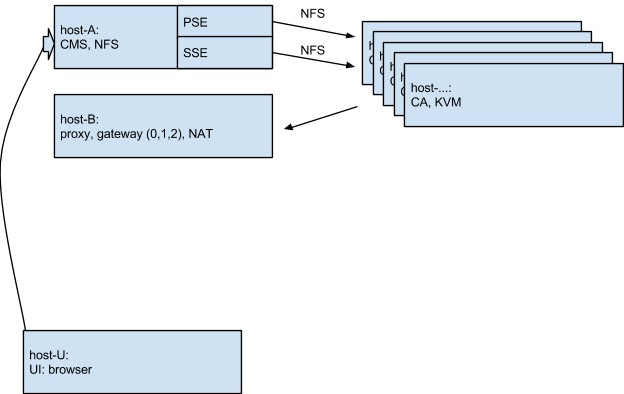
\includegraphics[width=\textwidth]{figures/hosts}
	\end{center}
	\caption{Hosts.}
	\label{fig:hardware:hosts}
\end{figure}



\section{Services Layout}
\label{sct:hardware:layout}
We recommend the following configuration:
\begin{description}
	\item[\host{A}] \acrshort{cms}, \acrshort{pse}, \acrshort{sse}
	\item[\host{B}] \acrshort{sq}, \acrshort{gwext}, \acrshort{gwint}
	\item[\host{C}, \host{D}, \dots] \acrshort{ca}
	\item[\host{U}] Administrator/User computer
\end{description}

\begin{figure}
	\begin{center}
		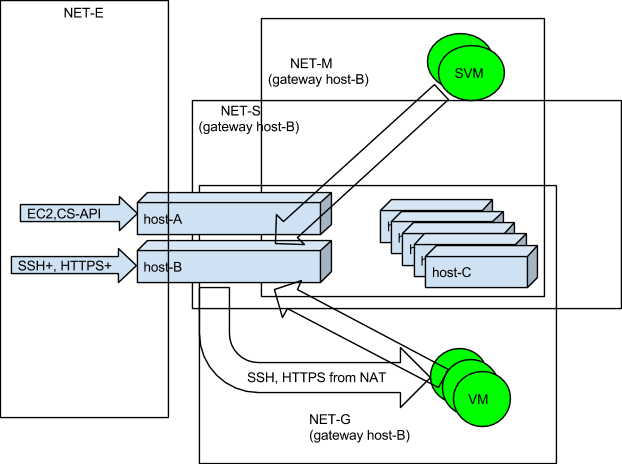
\includegraphics[width=\textwidth]{figures/layout}
	\end{center}
	\caption{Services layout.}
	\label{fig:hardware:layout}
\end{figure}

\section{Network Configuration}
\label{sct:hardware:network}

\subsection{Configuration via ``Basic Zone Network''}

If we are going to configure the network for \cstack\ using ``Basic Zone Network'', we need four preconfigured networks:
\begin{enumerate}
	\item \acrfull{nete}
	\item \acrfull{nets}
	\item \acrfull{netm}
	\item \acrfull{netg}
\end{enumerate}

\subsubsection{\acrfull{nete}}
External network is used for accessing to cloud through \acrshort{ec2api}, \acrshort{csapi} and selected virtual machines from internet/unsecured networks.
This network must be configured on \host{A} (for accessing to the \acrshort{ec2api} and \acrshort{csapi}) and on \host{B} (for access to virtual machines via \acrshort{nat}).

\subsubsection{\acrfull{nets}}
The storage network is used to provide access to storage pools for \acrshort{ca}s. 
It must be configured on \host{A} and on \acrshort{ca}s hosts (\host{C}, \host{D}, \dots).

\subsubsection{\acrfull{netm}}
The management network is used for communication between the \cstack\ components. 
All hosts must be able to connect to this network.

\subsubsection{\acrfull{netg}}
The guest network is used for communication between virtual machines and between virtual machines and external network, also it used for \acrshort{nat}-ing ports 22 and 443 to the external network.
\acrshort{netg} \acrshort{nat} rules must be configured on \host{B}.
At present time we use the following rules for port forwarding
\begin{lstlisting}
-A PREROUTING -d host-B -p tcp -m tcp --dport x443 -j DNAT --to-destination 10.1.2.x:443
-A PREROUTING -d host-B -p tcp -m tcp --dport x022 -j DNAT --to-destination 10.1.2.x:22
\end{lstlisting}
10.1.2.x is an IP of a virtual machine in \acrshort{netg}.
